
\chapter{Implementation}
\label{ch:Implementation}

To evaluate and refine the concept and integrate it into the \textsc{Vitruvius} framework, a prototype was implemented.
The implementation uses the \emph{eMoflon::IBeX} TGG framework (\cite{eMoflonIBeX_weidmann_incremental_nodate}, see \autoref{sec:Foundations:eMoflon}), which was originally developed as a set of plugins for the \emph{Eclipse} IDE. This made the development process challenging to a certain extent.
The prototype was written in Java-21 \cite{noauthor_jdk_21nodate}.

In the following, noteworthy aspects of the prototype implementation are described.
First, in \autoref{sec:Implementation:ChangesToVitruvius}, changes that have been made to \textsc{Vitruvius} to enable propagating sequences of changes at one go are described.
Section \ref{sec:Implementation:ChangesSequenceTemplates} explains details of the realization of \emph{Change Sequence Templates}, their instantiation, matching, and initialization.
Then, in \autoref{sec:Implementation:PatternMatchingProcess} details of the pattern matching process that is prescribed by eMoflon::IBeX to a certain extent are shown.
Section \ref{sec:Implementation:EnablingAttributeConstraints} describes how using attribute constraints has been enabled, and \autoref{sec:Implementation:Challenges} concludes by describing challenges with the IBeX framework that have emerged during the implementation of the prototype.

\section{Changes to \textsc{Vitruvius}}
\label{sec:Implementation:ChangesToVitruvius}
Since the concept requires retrieving a sequence of changes upon which TGG rules are matched, \textsc{Vitruvius}, which previously only supported propagating single \texttt{EChange}s one at a time, had to be modified.
That was done by adding methods to the 
\newline\texttt{ChangePropagationSpecification} interface that the \newline\texttt{TGGChangePropagationSpecification} included in this prototype implements, and changing the propagation functionality in \texttt{ChangePropagator}, both being part of the project \emph{Vitruv-Change}.

\paragraph{ChangePropagationSpecification} In the ChangePropagationSpecification interface, the two methods seen in \autoref{implChangePropSpec} are added.
\texttt{doeshandleNonAtomicChange} is added, by default returning \texttt{false} to ensure pre-existing ChangePropagationSpecification implementations' behaviour doesn't change and \texttt{propagateNonAtomicChange} isn't called if it is not implemented.
\texttt{propagateNonAtomicChange} is added and called by \texttt{ChangePropagator} (see \autoref{implChangePropagator}), to propagate a whole change sequence that is contained in the \texttt{VitruviusChange}.

\paragraph{ChangePropagator} In \texttt{ChangePropagator}, one method is modified and two methods are created to support propagating VitruviusChanges to ChangeSequenceTemplate implementations that implement \texttt{propagateNonAtomicChange} (see \autoref{implChangePropSpec}).
\texttt{propagateChanges} now calls propagateNonAtomicChange, too, which is largely based on the existing method \texttt{propagateSingleChange}. It is modified to only concern ChangePropagationSpecifications that handle non-atomic changes.
\newline It calls \texttt{propagateNonAtomicChangeForChangePropagationSpecification} on each registered ChangePropagationSpecification, which forwards the given \texttt{VitruviusChange} to those ChangePropagationSpecifications and collects their effects on their target models.
This is the entry point to the prototype.

\begin{figure}[H]
\centering
\begin{lstlisting}[language=java, caption={Added methods in \emph{ChangePropagationSpecification.xtend}}, captionpos=b, label=implChangePropSpec]
...
def boolean doesHandleNonAtomicChanges() { false }
def void propagateNonAtomicChange(
                        VitruviusChange<EObject> change, 
                        EditableCorrespondenceModelView<Correspondence> correspondenceModel,   
                        ResourceAccess resourceAccess) {
    // noop
}
\end{lstlisting}
\end{figure}

\begin{figure}[H]
\centering
\begin{lstlisting}[language=java, caption={Excerpts of changes to methods in \emph{ChangePropagator.xtend}, enabling change sequence propagation}, captionpos=b, label=implChangePropagator]
def private propagateChanges() {
		    val result = propagateNonAtomicChange()
			result += sourceChange.transactionalChangeSequence
                    .flatMapFixed[propagateSingleChange(it)]
            ...
}

def private List<PropagatedChange> propagateNonAtomicChange() {
    ...
    val propagationResultChanges = try {
        sourceChange.affectedEObjectsMetamodelDescriptors.flatMap [
            // we only want ChangePropSpecs that handle non-atomic changes
            changePropagationProvider.getChangePropagationSpecifications(it)
                .filter[it.doesHandleNonAtomicChanges()] => [
                    forEach[it.userInteractor = outer.userInteractor]
                ]
        ].toSet.flatMapFixed [
            propagateNonAtomicChangeForChangePropagationSpecification(sourceChange, it)
        ]
    }
    ...
}

def private propagateNonAtomicChangeForChangePropagationSpecification(
    VitruviusChange<EObject> change,
    ChangePropagationSpecification propagationSpecification
) {
    val transitiveChanges = modelRepository.recordChanges [
        propagationSpecification.propagateNonAtomicChange(change, 
                modelRepository.correspondenceModel,
                modelRepository)
    ]
    // Store modification information
    changedResources += transitiveChanges.flatMap[it.affectedEObjects]
            .map[eResource]
            .filterNull
    return transitiveChanges
}
\end{lstlisting}
\end{figure}

\section{Change Sequence Templates}
\label{sec:Implementation:ChangesSequenceTemplates}
In \autoref{sec:Concept:BackwardConversionPM:BackwardConversion}, the concept and structure of \emph{Change Sequence Templates} was described. This section presents noteworthy implementation details of the prototype.

In the prototype implementation, \texttt{ChangeSequenceTemplates} and \texttt{EChangeWrappers} have different states and roles in the pattern matching process. Those are illustrated in \autoref{fig:ChangeSeqTemplateInstanceDiagramDifferentStates}. The pattern conversion step produces a \texttt{ChangeSequenceTemplateSet}. The ChangeSequenceTemplates and their EChangeWrappers contained in that ChangeSequenceTemplateSet have an implicit parent/original role. They do not and will not hold any \texttt{EObject}s, they are templates to be copied and thus instantiated.

\begin{figure}
\centering
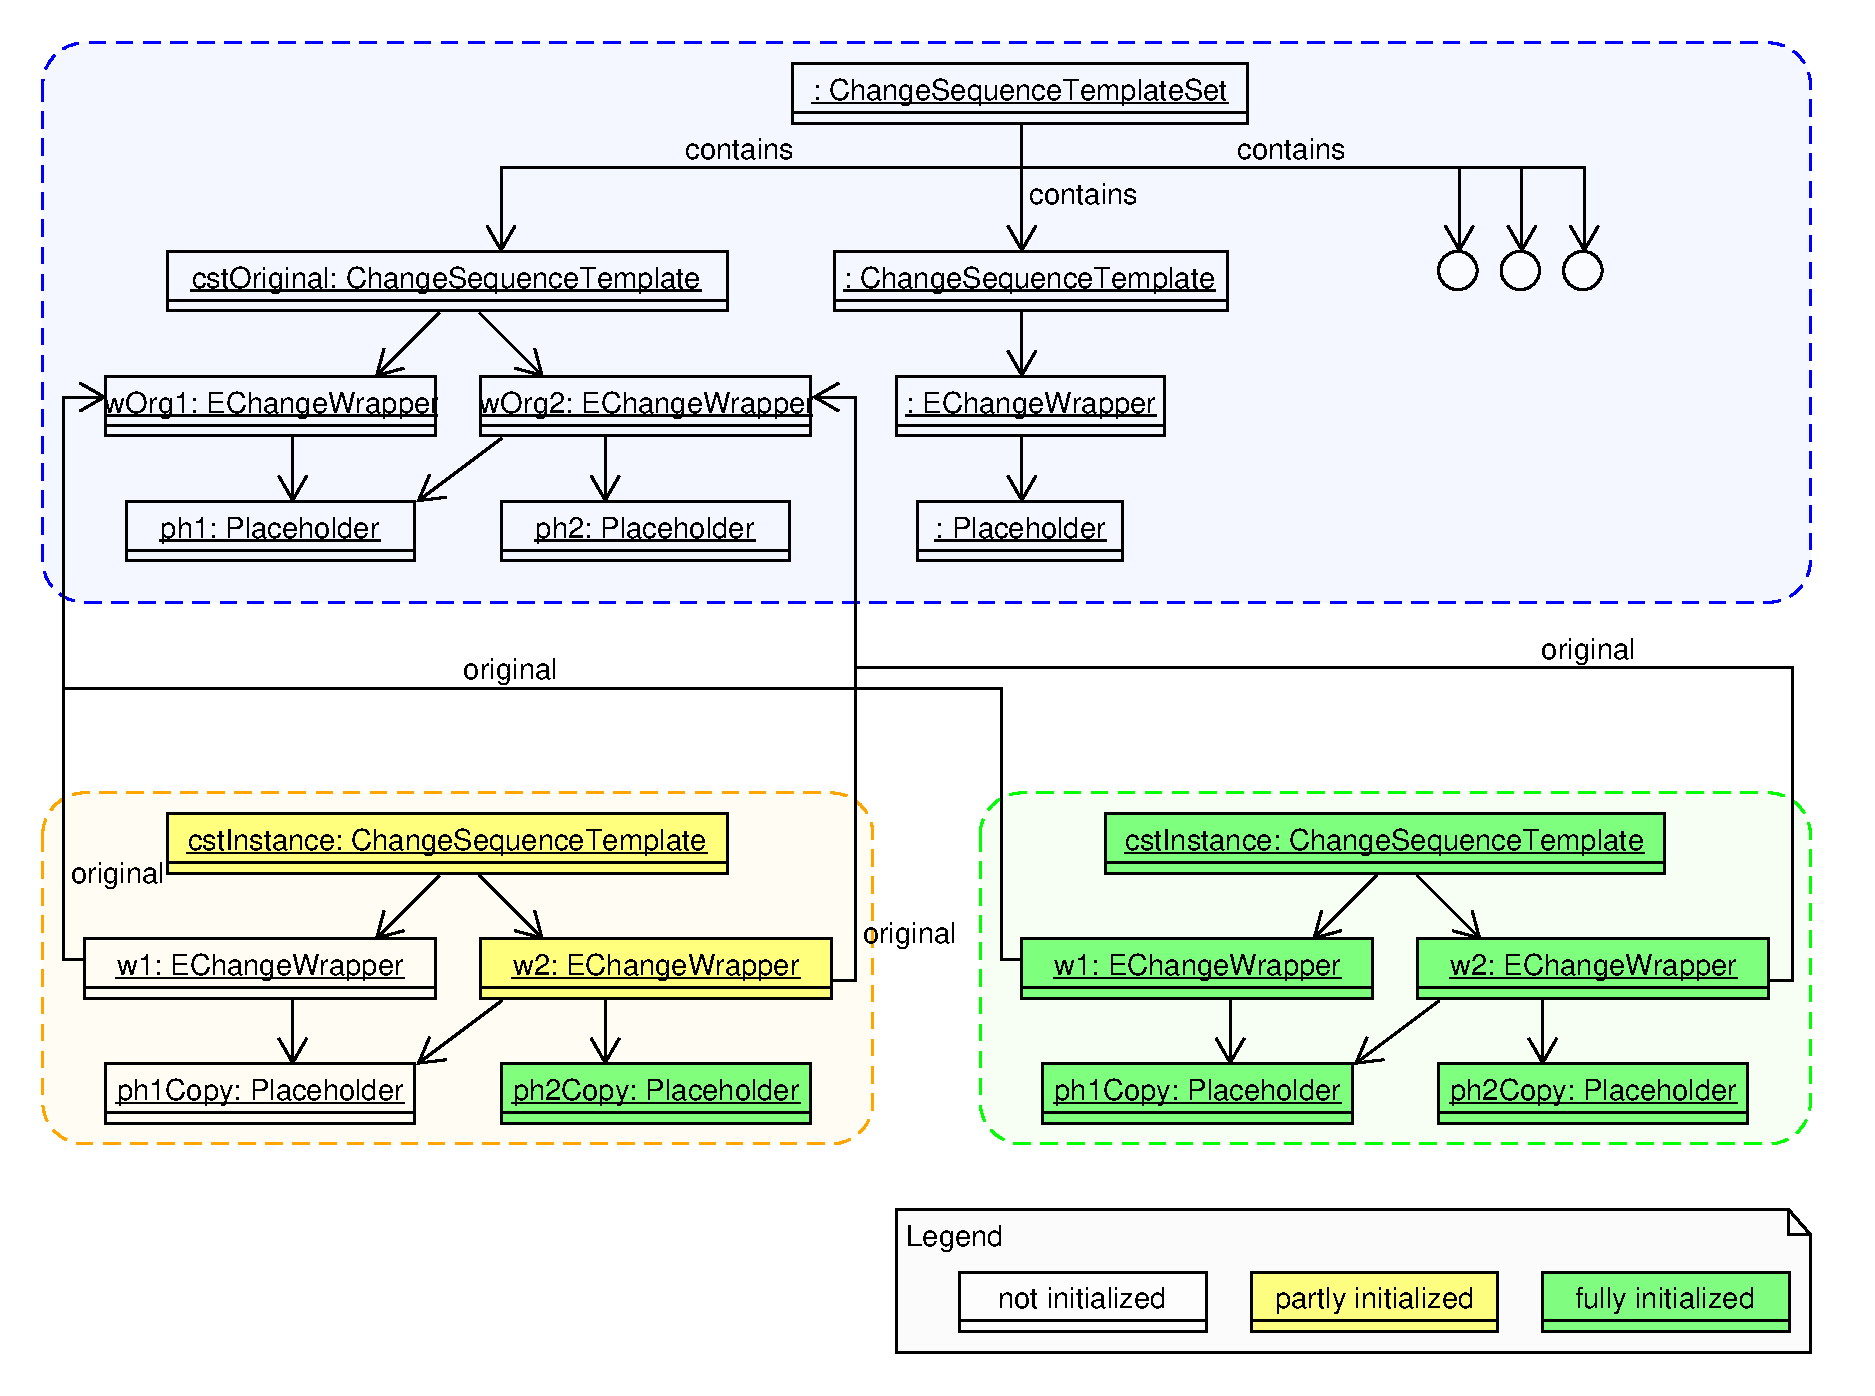
\includegraphics[width=15.5cm]{figures/ChangeSeqTemplateInstanceDiagramDifferentStates.pdf}
\caption[Different states and roles of \texttt{ChangeSequenceTemplate}s]{Different states and roles of \texttt{ChangeSequenceTemplate}s. The originals, which serve as templates for instantiating ChangeSequenceTemplates that serve an instance role, are shown in the blue box, along with the \texttt{ChangeSequenceTemplateSet} containing them. The orange box in the bottom left shows an instantiated (note the \emph{original} references) and partly initialized ChangeSequenceTemplate, where one EChangeWrapper is partly initialized and one placeholder is fully initialized. In the green box to the bottom right, the same ChangeSequenceTemplate is shown after it has been fully matched.}
\label{fig:ChangeSeqTemplateInstanceDiagramDifferentStates}
\end{figure}

For instantiation, \texttt{getAndInitRelevantChangeSequenceTemplatesByEChange} is called on a ChangeSequenceTemplateSet, returning one or more instances of each ChangeSequenceTemplate that contains an EChangeWrapper that is matchable to an EChange. For each matchable EChangeWrapper, one instance is created and initialized with the EChange, as can be seen in \autoref{implChangeSequenceTemplateSetGetAndInit}.
To reduce both runtime and complexity, a \texttt{HashMap} that maps \texttt{EChange} \texttt{EClass}es to the Set of ChangeSequenceTemplates that contain at least one EChangeWrapper of that type is used.

The ChangeSequenceTemplate instances created by \newline\texttt{getAndInitRelevantIbexPatternTemplatesByEChange} now each have one EChangeWrapper initialized fully. Because of the placeholder structure, this might indirectly initialize other EChangeWrappers \emph{partially} or \emph{fully}.
An EChangeWrapper is fully initialized if all of its \texttt{EObjectPlaceholder}s are holding an EObject.
Thus, at this point, some of the returned ChangeSequenceTemplates are partially or fully initialized (see \autoref{implChangeSequenceTemplateSetGetAndInit}).
After pattern matching, they are either fully initialized, indicating a successful green match, or discarded.

In the following, the mechanisms of matching and initializing EChangeWrappers are described, followed by an explanation of the copy mechanism.

\begin{figure}[H]
\centering
\begin{lstlisting}[language=java, caption={Change Sequence Template Instantiation in \texttt{ChangeSequenceTemplateSet}}, captionpos=b, label=implChangeSequenceTemplateSetGetAndInit]
public Set<ChangeSequenceTemplate> getAndInitRelevantChangeSequenceTemplatesByEChange(
        EChange<EObject> eChange) {
    Set<ChangeSequenceTemplate> partlyInitializedTemplates = new HashSet<>();
    for (ChangeSequenceTemplate changeSequenceTemplate : changeSequenceTemplatesByEChangeType
            .get(eChange.eClass())) {
        changeSequenceTemplate.getEChangeWrappers().stream()
            .filter(eChangeWrapper -> eChangeWrapper.matches(eChange))
            .forEach(eChangeWrapper -> {
                ChangeSequenceTemplate changeSequenceTemplateCopy = 
                        changeSequenceTemplate.deepCopy();
                changeSequenceTemplateCopy
                    .getThisInstancesEChangeWrapperFromParent(eChangeWrapper)
                    .initialize(eChange);
                partlyInitializedTemplates.add(changeSequenceTemplateCopy);
            });
    }
    return partlyInitializedTemplates;
}
\end{lstlisting}
\end{figure}


\subsection{Matching and initialization}
\label{sec:Implementation:MatchingAndInit}
The methods for matching and initializing an EChangeWrapper form a pair. They are similarly structured and intended to be called after one another.
First, \emph{matches} is called on an EChange, checking equality of the type of the given \texttt{EChange} and the EChangeWrappers \texttt{EChange} type, and, if present, all \texttt{EObject}s contained in placeholders of the EChangeWrapper. This flexibility in matching is needed because EChangeWrappers might be partly initialized by other EChangeWrappers of the same ChangeSequenceTemplates having been initialized before and sharing placeholders.
For different kinds of \texttt{EChange}s, different subclasses of EChangeWrapper are defined. Those hold different additional fields and placeholders for further \texttt{EObject}s that an \texttt{EChange} might contain. As subclasses differ in what they hold, matching and initializing an EChangeWrapper must be subclass-specific.
To realize that, both methods follow a similar concept: The \texttt{EChange} type, meaning its EClass, and the affectedEObject are handled in the abstract \texttt{EChangeWrapper} parent class by the methods \texttt{initialize} and \texttt{matches}. The additional matching checks and initialization are handled in subclasses that implement the abstract methods \texttt{initializeExtension} and \texttt{extendedDataMatches}, as shown in \autoref{implMatchingAndInit}.

\begin{figure}[H]
\centering
\begin{lstlisting}[language=java, caption={Matching and initialization in \texttt{EChangeWrapper}}, captionpos=b, label=implMatchingAndInit]
public boolean matches(EChange<EObject> eChange) {
    return  eChangeTypeAndAffectedEObjectMatches(eChange) && extendedDataMatches(eChange);
}
public void initialize(EChange<EObject> eChange) {
    this.setEChange(eChange);
    this.getAffectedElementPlaceholder().initialize(Util.getAffectedEObjectFromEChange(eChange));
    // delegate further initialization to subclasses
    this.isInitialized = true;
}

protected abstract void initializeExtension(EChange<EObject> eChange);
protected abstract boolean extendedDataMatches(EChange<EObject> eChange);

\end{lstlisting}
\end{figure}

\subsection{Copy mechanism}
\label{sec:Implementation:CopyMechanism}
As mentioned before, ChangeSequenceTemplate \emph{parents} are created by pattern conversion (\texttt{IbexPatternToChangeSequenceTemplateConverter}) and instantiated in the process of pattern matching.
This raises the need for a copy mechanism that keeps the ChangeSequenceTemplate's EChangeWrapper and placeholder structure.
Its implementation is shown in \autoref{implCSTdeepCopy}.
First, each EChangeWrapper is copied shallowly, meaning that the placeholders in the new EChangeWrappers remain the same as in their original. The new EChangeWrapper gets a reference to its original by setting the \texttt{original} field. A mapping of old to new EChangeWrappers is created.
Then, a mapping of old to new \texttt{Placeholders} is created and handed to each EChangeWrapper to replace their old placeholders with new ones.
Finally, a new ChangeSequenceTemplate is created via a copy constructor that takes the new EChangeWrappers and the map.
The map is used by the instance to be able to retrieve EChangeWrapper instances given an \texttt{original} EChangeWrapper, as is done in \autoref{implChangeSequenceTemplateSetGetAndInit} by calling \texttt{getThisInstancesEChangeWrapperFromParent}.

\begin{figure}[H]
\centering
\begin{lstlisting}[language=java, caption={Copy mechanism in \texttt{ChangeSequenceTemplate}}, captionpos=b, label=implCSTdeepCopy]
public ChangeSequenceTemplate deepCopy() {
        Collection<EChangeWrapper> newEChangeWrappers = new LinkedList<>();
        Map<EChangeWrapper, EChangeWrapper> oldToNewEChangeWrapperMap = new HashMap<>();
        for (EChangeWrapper changeWrapper : this.eChangeWrappers) {
            EChangeWrapper newEChangeWrapper = changeWrapper.shallowCopy();
            oldToNewEChangeWrapperMap.put(changeWrapper, newEChangeWrapper);
            newEChangeWrappers.add(newEChangeWrapper);
        }
        Map<EObjectPlaceholder, EObjectPlaceholder> oldToNewPlaceholders = newEChangeWrappers
                .stream()
                .flatMap(eChangeWrapper -> eChangeWrapper.getAllPlaceholders().stream())
                .distinct()
                .collect(Collectors.toMap(
                        eObjectPlaceholder -> eObjectPlaceholder,
                        eObjectPlaceholder -> new EObjectPlaceholder(eObjectPlaceholder
                                .getTggRuleNode())
                ));
        for (EChangeWrapper eChangeWrapper : newEChangeWrappers) {
            eChangeWrapper.replaceAllPlaceholders(oldToNewPlaceholders);
        }
        return new ChangeSequenceTemplate(this.tggRule, 
                this.iBeXContextPatternMap, newEChangeWrappers, oldToNewEChangeWrapperMap);;
    }
\end{lstlisting}
\end{figure}
% \section{Pattern Conversion}

\section{Pattern Matching Process}
\label{sec:Implementation:PatternMatchingProcess}
The implementation of the pattern matching process is considerably influenced by the synchronization algorithm and architecture of \emph{eMoflon::IBeX}, which is described in \autoref{sec:Foundations:eMoflon:syncProcess}.
This section describes the side of the process that concerns the pattern matching, which is driven by being able to correctly implement the method \texttt{updateMatches)} in \texttt{VitruviusBackwardConversionTGGEngine}.
% First, in \autoref{sec:Implementation:PatternMatchingProcess:Engine}, functionings of that class, especially the method \texttt{updateMatches}, are explained.
% In further subsections, details on dependencies of that class are described.
% That includes the \texttt{VitruviusChangePatternMatcher} (see \autoref{sec:Implementation:PatternMatchingProcess:GreenMatch}) and the \texttt{VitruviusChangeBrokenMatchMatcher} (see \autoref{sec:Implementation:PatternMatchingProcess:RedMatcher}).

\subsection{VitruviusBackwardConversionTGGEngine}
\label{sec:Implementation:PatternMatchingProcess:Engine}
This section describes functionality of the class \texttt{VitruviusBackwardConversionTGGEngine} that implements the pattern matcher interface of IBeX, called \texttt{IBlackInterpreter}
and thus serves as a partner to the \texttt{SYNC}-extending class \newline\texttt{VitruviusTGGChangePropagationIbexEntrypoint}.
The interesting parts are described in the following by elucidating noteworthy methods.

\paragraph{initPatterns} Implementing the \texttt{IContextPatternInterpreter} interface of IBeX, \newline\texttt{VitruviusTGGChangePropagationIbexEntrypoint} implements the method \texttt{initPatterns}.
This method is used to initialize the pattern matchers \texttt{VitruviusChangePatternMatcher} and \texttt{VitruviusChangeBrokenMatchMatcher}. Also, pattern conversion is triggered here, using \texttt{IbexPatternToChangeSequenceTemplateConverter}.

\paragraph{updateMatches}
As described in \autoref{sec:Foundations:eMoflon:syncProcess}, in \newline\texttt{VitruviusBackwardConversionTGGEngine}, the \texttt{updateMatches} method, shown in \autoref{implUpdateMatches} is called multiple times by \texttt{VitruviusTGGChangePropagationIbexEntrypoint} which extends the IBeX class \texttt{SYNC} that, along with further parent classes, defines the synchronization algorithm of IBeX. In the following, the handle \texttt{SYNC} is used in descriptions of the process.
Between each call and the next, the triple graph might have been changed by \texttt{SYNC}. Matches might have been applied or revoked, changing the correspondence graph, the protocol, and the target model.
First, so-called \emph{consistency matches} are initialized, if not already present, by loading the \emph{protocol} that stores rule applications from previous runs and transforming them to \texttt{VitruviusConsistencyMatch}es. That is a class implementing the IBeX interface \texttt{ITGGMatch} and is used in the prototype to represent broken matches or intact matches that have been loaded from the protocol file.
For unknown reasons, this initialization is not done by IBeX itself.
To avoid recalculating matches each time updateMatches is called, \texttt{createForwardMatchesIfNotAlreadyPresent} creates green matches one time and saves the result in a class field for further calls.
However, since some of these matches might have been already applied, the remaining green matches that have not already been applied and whose green nodes are not already covered by a match having been applied prior to the current run of \texttt{updateMatches} are calculated in \texttt{getMatchesThatHaventBeenAppliedAndAreStillIntact} (see \autoref{implGetMatchesThatHaventBeenAppliedAndAreStillIntact}).
\texttt{VitruviusBackwardConversionTGGEngine} knows about matches that have been applied by implementing the IBeX interface \texttt{IbexObserver} and observing \texttt{MATCHAPPLIED} \texttt{ObservableEvent}s.
The filtered set of matches is then again thinned out twice: First, each match undergoes context matching, as described in \autoref{sec:Concept:BackwardConversionPM:BlackMatching}. Then, match selection, as described in \autoref{sec:Concept:PatternSelection} is applied, before handing the remaining matches to \texttt{SYNC}.
After having handled the additive matches, broken matches that have not been handled yet are determined using the \texttt{VitruviusChangeBrokenMatchMatcher} (see \autoref{sec:Implementation:PatternMatchingProcess:RedMatcher} and reported to \texttt{SYNC}.
Finally, in \texttt{repairUnrepairedBrokenMatches} (see \autoref{implRepairUnrepairedBrokenMatches}), broken matches newly invalidated by the \texttt{RedInterpreter} used by \texttt{SYNC} are tried to be repaired, possibly creating and applying new additive matches (see \autoref{sec:Concept:RedMatching:Repair}).

\begin{figure}[H]
\centering
\begin{lstlisting}[language=java, caption={Copy mechanism in \texttt{ChangeSequenceTemplate}}, captionpos=b, label=implUpdateMatches]
@Override
public void updateMatches() {
    initializePreexistingConsistencyMatchesIfNotAlreadyPresent();

    createForwardMatchesIfNotAlreadyPresent();
    Set<VitruviusBackwardConversionMatch> remainingMatches = 
            getMatchesThatHaventBeenAppliedAndAreStillIntact();

    matchContext_flatten_andHandToSYNC(remainingMatches);

    Set<VitruviusConsistencyMatch> brokenMatches = getBrokenMatches();
    brokenMatches.forEach(brokenMatch -> {
        this.iMatchObserver.removeMatch(brokenMatch);
    });

    // Repair matches that are broken and have not been repaired by shortcut rules
    if (ibexOptions.repair.useShortcutRules()) {
        throw new IllegalStateException("Using shortcut rules not supported yet: 
            Need to filter out repaired matches from the broken matches...");
    }
    repairUnrepairedBrokenMatches();
}
\end{lstlisting}
\end{figure}

\paragraph{getMatchesThatHaventBeenAppliedAndAreStillIntact} The method \newline\texttt{getMatchesThatHaventBeenAppliedAndAreStillIntact}, which is depicted in \autoref{implGetMatchesThatHaventBeenAppliedAndAreStillIntact}, helps ensure that matches given to \texttt{SYNC} have not been applied before and are not containing green nodes whose matched-to \texttt{EObject} is already covered by another match having been applied before.
As mentioned before, matches that have been applied are known because \texttt{VitruviusBackwardConversionTGGEngine} implements the IBeX interface \texttt{IbexObserver}. 
From these already applied matches, the \texttt{EObject}s covered by green nodes of the TGGRule belonging to the match are collected.
Then, the green matches that are to be filtered are sorted out if they were already applied or would cover one of these previously collected, already covered \texttt{EObject}s.

\begin{figure}[H]
\centering
\begin{lstlisting}[language=java, caption={Match filtering in \texttt{VitruviusBackwardConversionTGGEngine}}, captionpos=b, label=implGetMatchesThatHaventBeenAppliedAndAreStillIntact]
private Set<VitruviusBackwardConversionMatch> getMatchesThatHaventBeenAppliedAndAreStillIntact() {
        Set<EObject> createdEObjectsAlreadyCovered = this.matchesThatHaveBeenApplied.stream()
                .map(match -> (VitruviusBackwardConversionMatch) match)
                .flatMap(match -> match.getEObjectsCreatedByThisMatch().stream())
                .collect(Collectors.toSet());

        return this.matchesFound.stream()
                .filter(match -> !this.matchesThatHaveBeenApplied.contains(match))
                .filter(match -> match.getEObjectsThisMatchWouldCreate().stream()
                        .noneMatch(createdEObjectsAlreadyCovered::contains))
                .collect(Collectors.toSet());
    }
\end{lstlisting}
\end{figure}

\paragraph{repairUnrepairedBrokenMatches} The method \texttt{repairUnrepairedBrokenMatches} (see \autoref{implRepairUnrepairedBrokenMatches}) tries to repair broken matches detected by \texttt{VitruviusChangeBrokenmatchMatcher} and invalidated by \texttt{IbexRedInterpreter}.
It does so by trying to repair broken matches using the \texttt{UnrepairedBrokenMatchOldChangesRetriever} to generate a new change sequence from those green nodes and edges of the broken matches that are still mapped to \texttt{EObject}s (see \autoref{fig:impl:brokenMatches} for an example).
This new change sequence is extended by adding all \texttt{EChange} that were left unmatched by the pattern matching of the \enquote{main} change sequence, the one that had started the change propagation process, that have not already been applied. This enables matches overspanning both change sequences to be possible.
The unmatched \texttt{EChange}s from the \enquote{main} change sequence are appended at the \emph{end} of the new change sequence to not distort the application of the distance heuristic (see \autoref{sec:Concept:PatternSelection} and \autoref{sec:Foundations:ComplexChangeDetection}).
In the example in \autoref{fig:impl:brokenMatches}, the \texttt{EChange} representing the creation of Y is in the main change sequence, and all \texttt{EObject}s that are referenced by green nodes (and their references) in the bottom graph get \texttt{EChange}s created in the new change sequence.
The resulting change sequence is given to a new \texttt{VitruviusChangePatternMatcher}, which calculates new matches.
These new matches are stored globally for \texttt{updateMatches} to hand them to \texttt{SYNC}.
Finally, the new matches are context-matched, coverage-flattened, and handed to \texttt{SYNC}, in case the current call to \texttt{updateMatches} and \texttt{repairUnrepairedBrokenMatches} was the last.

\begin{figure}
\centering
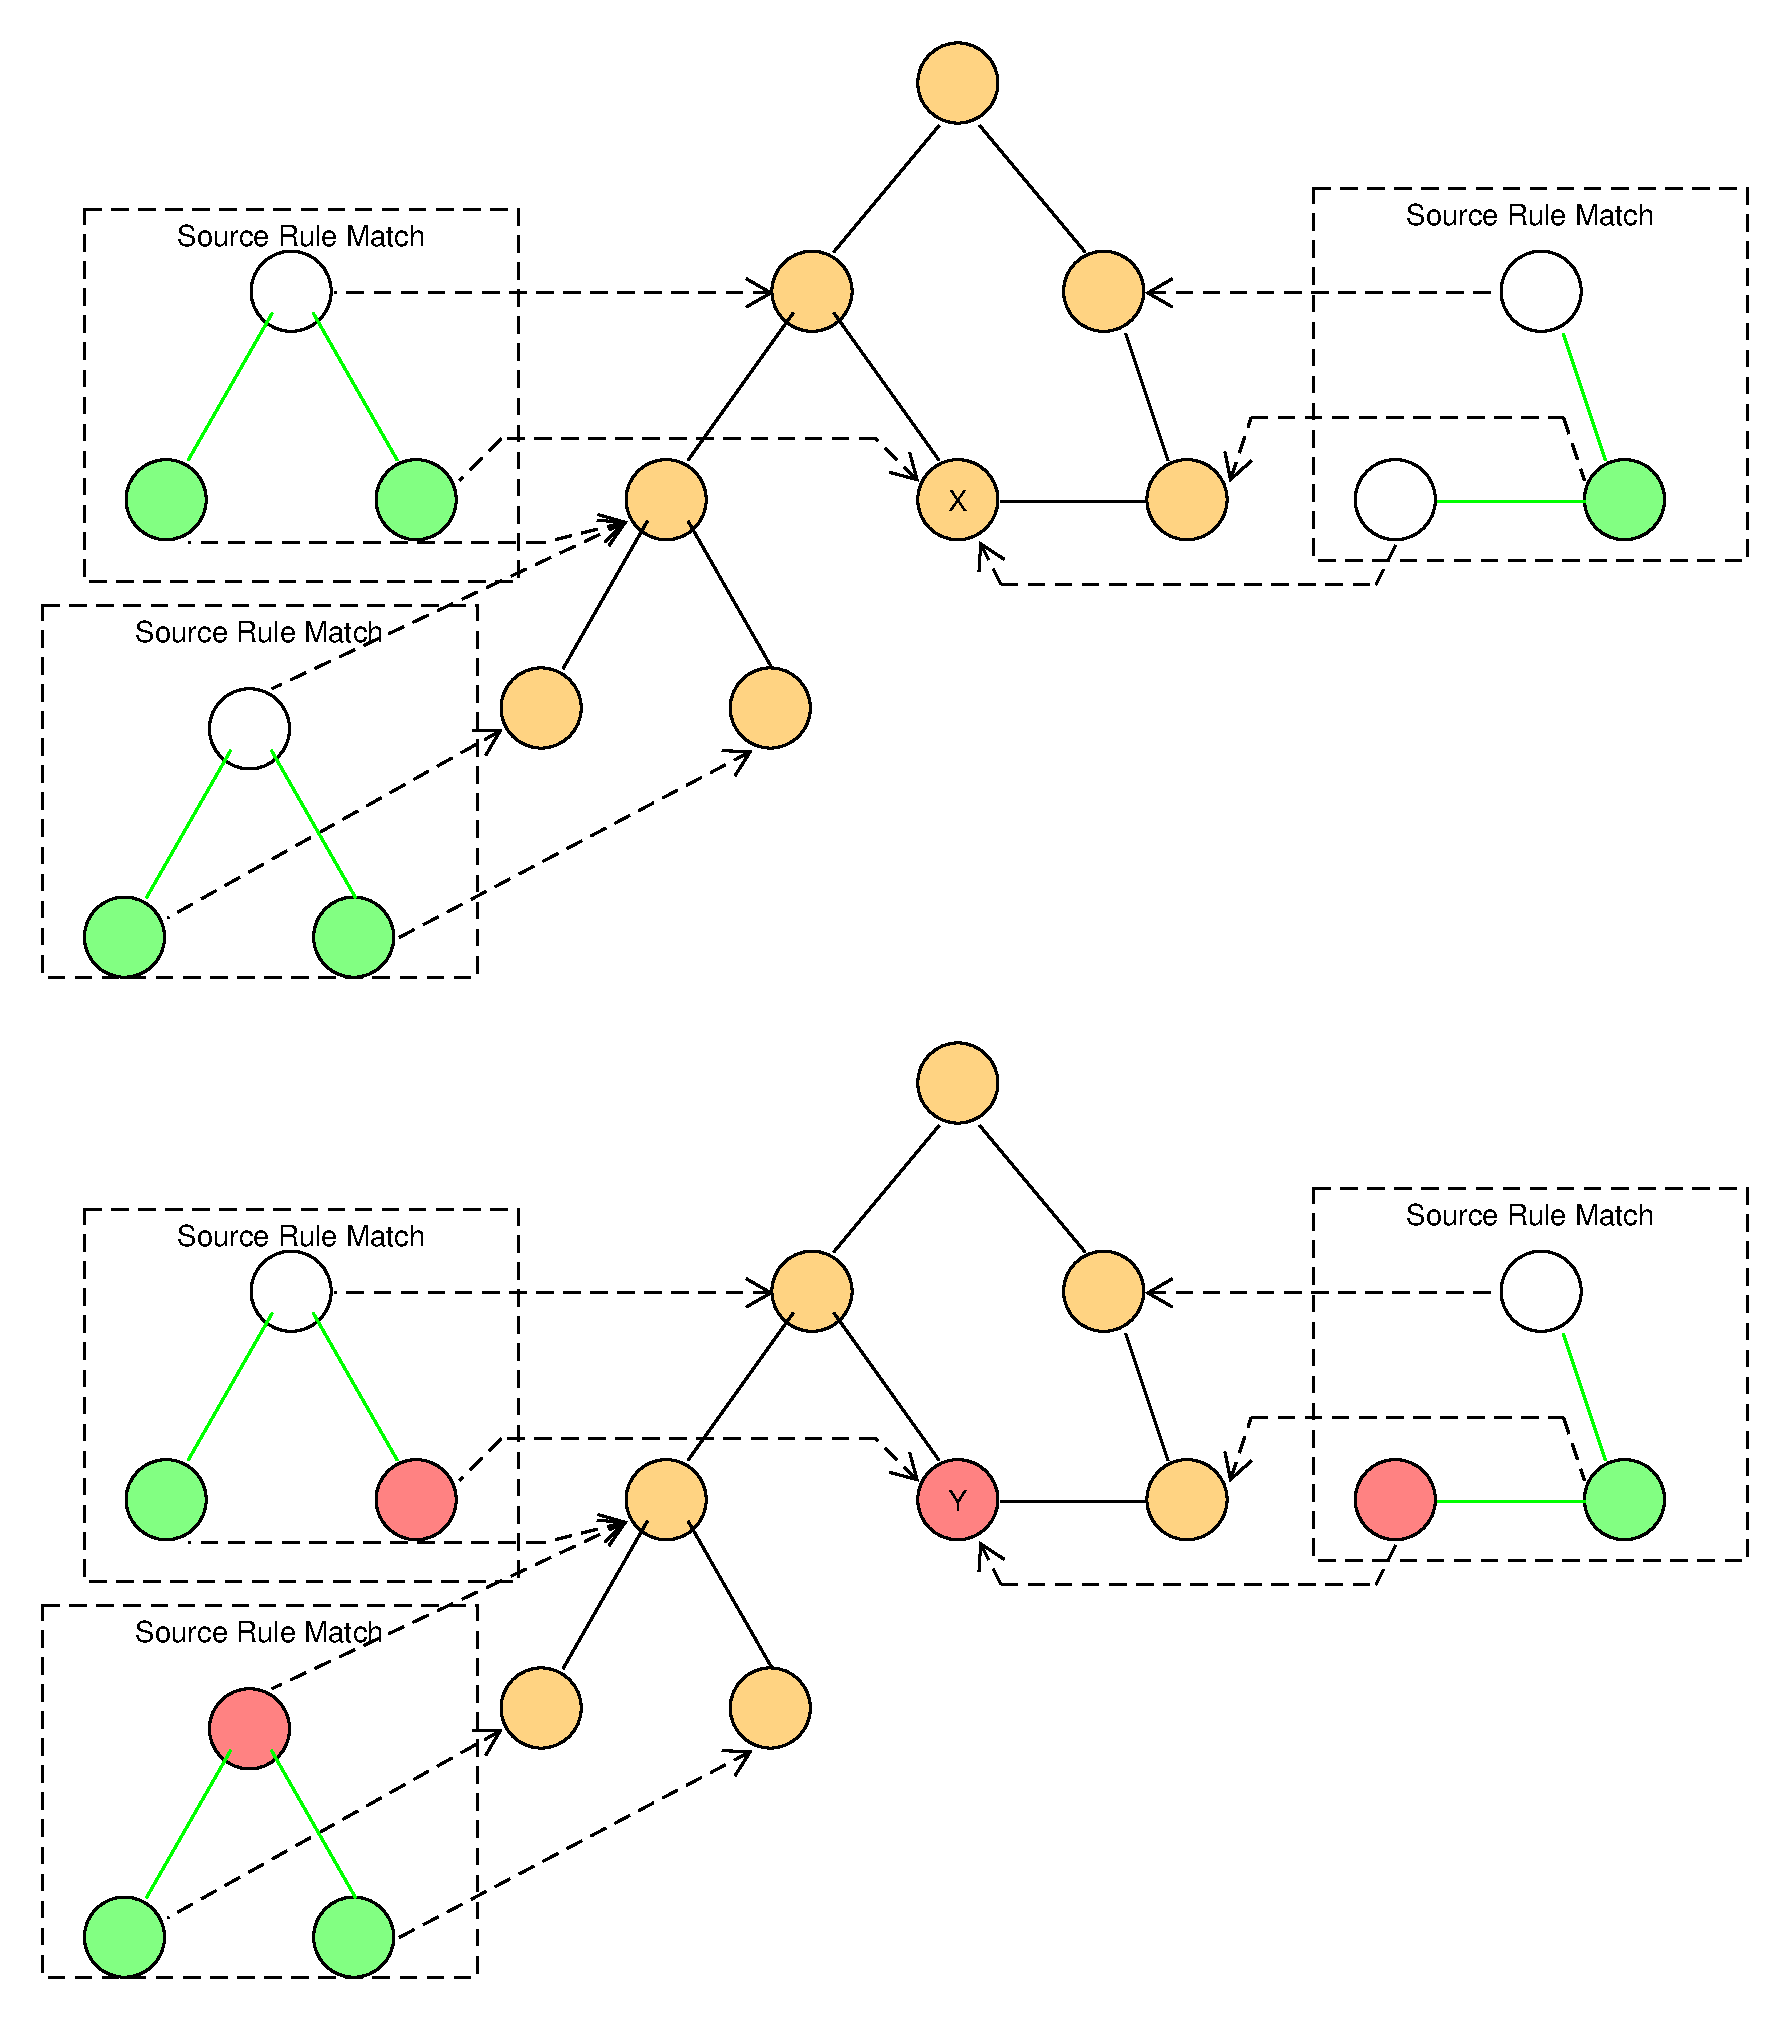
\includegraphics[width=16cm]{figures/brokenMatchExample.pdf}
\caption[Broken matches example]{TGG rule matches becoming broken after X is replaced by Y. All three rule matches are broken, and nodes remaining green in the bottom graph are now \enquote{free} to be covered by another rule match.}
\label{fig:impl:brokenMatches}
\end{figure}


\begin{figure}[]
\centering
\begin{lstlisting}[language=java, caption={repair handling in \texttt{VitruviusBackwardConversionTGGEngine}}, captionpos=b, label=implRepairUnrepairedBrokenMatches]
private void repairUnrepairedBrokenMatches() {
    Set<VitruviusConsistencyMatch> unrepairedAndUntriedBrokenMatches = this.vitruviusTGGIbexRedInterpreter.getRevokedRuleMatches().stream()
            .map(match -> (VitruviusConsistencyMatch) match)
            .filter(match -> !matchesThatHaveBeenTriedToRepair.contains(match))
            .collect(Collectors.toSet());
    if (unrepairedAndUntriedBrokenMatches.isEmpty()) {
        return; // no point
    }

    List<EChange<EObject>> newChangeSequence = new UnrepairedBrokenMatchOldChangesRetriever(
            this.observedOperationalStrategy.getResourceHandler(), 
            this.ibexOptions.tgg.flattenedTGG().getRules().stream()
                    .filter(tggRule -> !tggRule.isAbstract())
                    .collect(Collectors.toSet()),
            unrepairedAndUntriedBrokenMatches, propagationDirection
            ).createNewChangeSequence();
    newChangeSequence.addAll(vitruviusChangePatternMatcher.getUnmatchedEChanges());
    VitruviusChangePatternMatcher newVitruviusChangePatternMatcher = 
        new VitruviusChangePatternMatcher(
                VitruviusChangeFactory.getInstance()
                        .createTransactionalChange(newChangeSequence),
                changeSequenceTemplateSet
    );
    Set<VitruviusBackwardConversionMatch> newMatches = 
            newVitruviusChangePatternMatcher.getAdditiveMatches(propagationDirection);
    matchesThatHaveBeenTriedToRepair.addAll(unrepairedAndUntriedBrokenMatches);
    this.matchesFound.addAll(newMatches);
    matchContext_flatten_andHandToSYNC(newMatches);
}
\end{lstlisting}
\end{figure}

\subsection{Broken matches detection}
\label{sec:Implementation:PatternMatchingProcess:RedMatcher}
The \texttt{VitruviusChangeBrokenMatchMatcher} implements what is described in \autoref{sec:Concept:RedMatching:Implicit} and \autoref{sec:Concept:RedMatching:Explicit}.
However, the prototype has one limitation to that: \texttt{EList} indices are not stored in the protocol.
This means that the detection of \textsc{RemoveEReference} is not complete, because in case an element occurs twice in the list, the rule application match where that list insertion was marked with create nodes and edges is ambiguous.
Because of that, removing elements in lists that occur there more than once is not supported by the prototype.

\section{Enabling Attribute Constraints}
\label{sec:Implementation:EnablingAttributeConstraints}
As described in \autoref{sec:Foundations:eMoflon:attributeConditions}, eMoflon::IBeX supports defining attribute constraints to specify relationships between attributes of corresponding \texttt{EObject}s.
Because IBeX isn't designed as a library but as an Eclipse plugin, this was realized via class loading and the \emph{Java Reflection API}, which is shown in \autoref{implEnablingAttributeConstraints}.
The user must have defined custom attribute constraints in the default factory for that, which is \newline\texttt{UserDefinedRuntimeTGGAttrConstraintFactory}. That Class, although auto-generated in the process of an eMoflon build, always is contained in the same package, namely\newline
\texttt{org.emoflon.ibex.tgg.operational.csp.constraints.factories.<<projectName>>}. \newline
It is loaded and then instantiated and handed to IBeX.


\begin{figure}
    \centering
    \begin{lstlisting}[language=java, caption={Enabling Attribute Constraints in \texttt{VitruviusTGGChangePropagationRegistrationHelper}}, captionpos=b, label=implEnablingAttributeConstraints]
    private void tryToFindAndAddUserDefinedAttributeConstraints(IbexOptions ibexOptions) {
        try {
            //class loader should have access to this CL's classes as well as the ibex project
            Class userDefinedConstraintFactoryClass = new SimpleNameSupportingURLClassLoader(
                    new URL[]{new File(ibexProjectPath, "/bin").toURI().toURL()},
                    this.getClass().getClassLoader())
                    .loadClass("org.emoflon.ibex.tgg.operational.csp.constraints.factories." 
                            + ibexOptions.project.name().toLowerCase() 
                            + ".UserDefinedRuntimeTGGAttrConstraintFactory");
            ibexOptions.csp.userDefinedConstraints((RuntimeTGGAttrConstraintFactory)    
                    userDefinedConstraintFactoryClass.getConstructor().newInstance());
        } catch (MalformedURLException | InvocationTargetException | InstantiationException | 
                IllegalAccessException | NoSuchMethodException e) {
            logger.warn("Couldn't load UserDefinedRuntimeTGGAttrConstraintFactory");
        }
    }
    \end{lstlisting}
\end{figure}


\section{Challenges with the IBeX Framework}
\label{sec:Implementation:Challenges}

During the implementation of the prototype in eMoflon, a number of issues with the IBeX framework occurred, some of which could be dealt with, while others could not.
Especially the proxy issue, which had an impact on the evaluation results (see \autoref{sec:Evaluation:Results:G1}), artificially restricts the capabilities of the prototype, preventing rule applications that otherwise would be functioning.

\subsection{Solved Issues}
\label{sec:Implementation:Challenges:solved}

Some issues with the IBeX framework could be solved by overriding classes and methods from the framework. Some of these issues are bugs, others are a lacking of access to data required by the prototype implementation.
\paragraph{SmartEMF} On their website, the eMoflon developers describe \emph{SmartEMF} as a \enquote{High-performance EMF reimplementation complying with EMF interfaces} \cite{noauthor_emoflonibex_nodate}.
However, parts of the implementation do not comply with the EMF interfaces, which produced problems while testing the prototype.
One of those is \texttt{org.emoflon.smartemf.persistence.AdapterList}.

\paragraph{org.emoflon.smartemf.persistence.AdapterList} is a SmartEMF implementation of an EMF \texttt{EList<Adapter>}.
Because its internal representation is a \texttt{LinkedHashSet}, which doesnt implement \texttt{List} functions, methods like \texttt{get(int index)}, \texttt{add(int index, Adapter element)} or \texttt{indexOf(Object o)}, which have to be implemented to comply with the \texttt{EList} interface, miss data to return something meaningful. Thus, the developers of SmartEMF chose to throw an \texttt{UnsupportedOperationException} wherever these methods are called.
In preparing the evaluation, such a call occurred while loading model elements.
This issue was fixed in the \texttt{tools.vitruv.dsls.tgg.emoflonintegration.ibex.smartEmfFix} package by extending \texttt{AdapterList} with the \texttt{AdapterListFixed} class, overriding the aforementioned \texttt{indexOf} and \texttt{add} methods. \texttt{indexOf} always returns $0$, and \texttt{add} is implemented as a noop. This fixed the problem but should be kept in mind in case any persistence issue arises.
The \texttt{AdapterListFixed} was \enquote{injected} by also overriding the \texttt{SmartEMFResource} and the \texttt{SmartEMFResourceFactoryImpl} classes and registering the latter as the default \texttt{ResourceFactory} for the resourceSet of \texttt{VitruviusBackwardConversionTGGEngine}.

\paragraph{org.emoflon.ibex.tgg.operational.repair.strategies.AttributeRepairStrategy} is an IBeX class that enforces attribute constraints on matches. However, it also tries to enforce these on matches that are not fully matched, meaning that some nodes are not mapped to \texttt{EObject}s, which then results in a \texttt{NullPointerException}.
This has been fixed by extending the \texttt{AttributeRepairStrategy} with \texttt{FixedAttributeRepairStrategy} in the \newline
\texttt{tools.vitruv.dsls.tgg.emoflonintegration.ibex} package. There, the \texttt{repair} method was overridden and a \texttt{null} check added.
Similar to the \texttt{AdapterList} issue, the \newline\texttt{FlexibleSeqRepair} class, extending 
\newline\texttt{org.emoflon.ibex.tgg.operational.repair.SeqRepair}, was created to inject the \newline\texttt{FixedAttributeRepairStrategy}.

\paragraph{paranoid modifications} In the \texttt{VitruviusBackwardConversionTGGEngine}, which implements the \texttt{IBlackInterpreter} interface, the 
\texttt{getProperties} method can be overridden to, among others, set the \texttt{needs\_paranoid\_modifications} property.
While conducting the evaluation, it turned out that both states are needed.
For deleting changes, \newline
\texttt{needs\_paranoid\_modifications} being set to false leads to an \newline
\texttt{UnsupportedOperationException} being thrown in the UML EMF implementation. \newline
For additive changes, \texttt{needs\_paranoid\_modifications} being set to true makes the serialization faulty, losing some references that look like they are serialized but aren't deserialized.
This issue was again fixed by setting \texttt{needs\_paranoid\_modifications} to \texttt{false} by default and extending an IBeX class, in this case \texttt{IbexRedInterpreter}. The extending class, \texttt{VitruviusTGGIbexRedInterpreter}, overrides the \texttt{revoke(\dots)} method where it sets \texttt{needs\_paranoid\_modifications} temporarily to \texttt{true}, as can be seen in \autoref{implNeedsParanoidMod}.

\begin{figure}[H]
\centering
\begin{lstlisting}[language=java, caption={Source Model Serialization}, captionpos=b, label=implNeedsParanoidMod]
@Override
public void revoke(Set<EObject> nodesToRevoke, Set<EMFEdge> edgesToRevoke) {
    patternMatcher.setNeeds_paranoid_modificiations(true);
    super.revoke(nodesToRevoke, edgesToRevoke);
    patternMatcher.setNeeds_paranoid_modificiations(false);
}
\end{lstlisting}   
\end{figure}

\subsection{Unsolved Issues}
\label{sec:Implementation:Challenges:unsolved}
Unfortunately, some issues with eMoflon::IBeX could not be solved. As mentioned before, this distorts the evaluation results, which is also discussed in the evaluation chapter (\autoref{ch:Evaluation}).
In the following, these issues are described, as well as the reasons why they could not be solved.

\paragraph{Unresolved proxies} The proxy problem appeared in the process of the evaluation.
Some \texttt{TGGRules} contained nodes and/or references whose \texttt{type} attribute, which references the \texttt{EClass} or \texttt{EReference} that a node or an edge represents, was a \emph{proxy} (see \autoref{sec:Foundations:MDSE}), indicating that this metamodel element could not be loaded or has been unloaded.
These rules could be translated to \texttt{ChangeSequenceTemplates} by the prototype but not be matched to a \texttt{VitruviusChange}, because the proxy \texttt{EClass}es and \texttt{EReference}s could not be matched successfully to the \texttt{EObject}s' \texttt{EClass}es and the \texttt{EReference}s held by the \texttt{EChange}s.
They, however, were no proxies, which indicates that the problem does not lie with the model or its serialization being faulty but rather with the IBeX framework. 
All attempts to solve this problem failed, and since at the present time development of the IBeX framework is discontinued, a solution is likely only to be found by either forking the framework or moving to another, e.g., \emph{eMoflon::neo} \cite{weidmann_emoflonneo_nodate}.

\paragraph{Correspondence Model Serialization} Another issue that also occurred while conducting the evaluation concerned IBeX's serialization of the correspondence model.
This issue is illustrated with an example, as can be seen in \autoref{implSrcModelSerialization} and \autoref{implCorrGraphSerialization}.
In a situation where a many-valued reference has two or more values, a deletion of any but the last value results in the correspondence model serialization being corrupted. That is because, as can be seen in \autoref{implCorrGraphSerialization}, correspondence entries reference source and target entries by pointing at indexes in the respective model serialization files.
Deleting the first \texttt{members} entry named \enquote{constructer} in \autoref{implSrcModelSerialization} leads to the \texttt{source} entry in \autoref{implCorrGraphSerialization} now pointing to the formerly second, but now first \texttt{members} entry in \autoref{implSrcModelSerialization}, that is called \enquote{methed}.
In this case, IBeX won't even load the correspondence model, because the type checking of \texttt{JavaConstructorToOperation} fails, since it expects a \texttt{Constructor} as source but gets a \texttt{ClassMethod}.
If the first member were also a member, this corruption would be silent.
Like with the unresolved proxies problem, this might be solved by using another framework or implementing an alternative serialization solution that does not relate objects by position but, e.g., by ID.

\begin{figure}[H]
\centering
\begin{lstlisting}[language=xml, caption={Source Model Serialization}, captionpos=b, label=implSrcModelSerialization]
 <classifiers xsi:type="classifiers:Class" name="kless">
     <members xsi:type="members:Constructor" name="constructer">
        <parameters xsi:type="parameters:OrdinaryParameter" name="parrametr"/>
     </members>
     <members xsi:type="members:ClassMethod" name="methed">
        <parameters xsi:type="parameters:OrdinaryParameter"/>
     </members>
     <members xsi:type="members:Field" name="myField"/>
 </classifiers>
\end{lstlisting}     
\end{figure}

\begin{figure}[H]
\centering
\begin{lstlisting}[language=xml, caption={Correspondence Model Serialization},captionpos=b, label=implCorrGraphSerialization]
 <Java2Uml:JavaConstructorToOperation>
     <target xsi:type="uml:Operation" href="uml_instance.model#/0/@packagedElement.0/@ownedOperation.0"/>
     <source xsi:type="members:Constructor" href="java_instance.model#//@compilationUnits.0/@classifiers.0/@members.0"/>
 </Java2Uml:JavaConstructorToOperation>
\end{lstlisting}       
\end{figure} 
